\chapter{Trigonométrie}
\thispagestyle{fancy}

\vspace{-0.5cm}
\section{Cercle trigonométrique et radian}

\subsection{Le cercle trigonométrique}

    \begin{minipage}{0.65\linewidth}
        \begin{bdefi}
            Sur un cercle, on appelle \grasInDef{sens direct, sens positif ou sens trigonométrique} le sens contraire des aiguilles d'une montre.
        \end{bdefi}
    
        \begin{bdefi}
            Dans le plan muni d'un repère orthonormé \Rij  et orienté dans le sens direct, le \grasInDef{cercle trigonométrique} est le cercle de centre O et de rayon 1.
        \end{bdefi}
    \end{minipage} \hfill
    \begin{minipage}[c]{0.35\linewidth}
        \psset{xunit=2cm,yunit=2cm,algebraic=true,dimen=middle,dotstyle=o,dotsize=5pt 0,linewidth=0.8pt,arrowsize=3pt 2,arrowinset=0.25}
        \begin{pspicture*}(-1.2,-1.2)(1.8,1.5)
        \psaxes[labelFontSize=\scriptstyle,xAxis=true,yAxis=true,labels=none,Dx=1,Dy=1,ticksize=-2pt 0,subticks=1]{->}(0,0)(-1.2,-1.2)(1.8,1.5)
        \pscircle[linewidth=0.8pt,linecolor=ForestGreen](0.,0.){2}
        \parametricplot[linewidth=1.2pt,linecolor=red]{0.2836313716099023}{1.2179063232586265}{1.*1.3698332060350076*cos(t)+0.*1.3698332060350076*sin(t)+0.|0.*1.3698332060350076*cos(t)+1.*1.3698332060350076*sin(t)+0.}
        \rput[tl](1.01,1.1){\footnotesize \red{Sens Direct}}
        \psline[linewidth=1.2pt,linecolor=blue]{->}(0.,0.)(1.,0.)
        \psline[linewidth=1.2pt,linecolor=blue]{->}(0.,0.)(0.,1.)
        \rput[tl](0.41,-0.1){\footnotesize $\blue{\vv{i}}$}
        \rput[tl](-0.17,0.55){\footnotesize $\blue{\vv{j}}$}
        \psline[linewidth=2.pt,linecolor=red](0.4734296463271147,1.2854210914461963)(0.5317198467755907,1.2004882024713655)
        \psline[linewidth=2.pt,linecolor=red](0.4734296463271147,1.2854210914461963)(0.5924995182352584,1.2882810612464408)
        \rput[tl](0.8,0.9){\Large \red{+}}
        \begin{scriptsize}
        %\psdots[dotsize=4pt 0,dotstyle=*,linecolor=darkgray](0.,0.)
        \rput[bl](-0.17737632025386682,-0.1434178664701735){O}
        \end{scriptsize}
        \end{pspicture*}
        %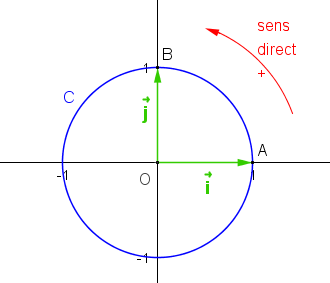
\includegraphics[scale=0.7]{01-02-01.png}
    \end{minipage}
    \vspace{-0.5cm}
    \subsection{Enroulement d'une droite autour du cercle trigonométrique}
    
    \begin{minipage}{0.65\linewidth}
        Dans un repère orthonormé \Rij), on considère le cercle trigonométrique et une droite (AC) tangente au cercle en A et orientée telle que $(A ; \vv{j})$ soit un repère de la droite.\\
        Si l'on \guillemets{enroule} la droite autour du cercle, on associe à tout point $N$ d'abscisse $x$ de la droite orientée un unique point $M$ du cercle.\\
        La longueur de l'arc $\wideparen{AM}$ est ainsi égale à la longueur AN.
    \end{minipage} \hfill
    \begin{minipage}[c]{0.35\linewidth}
        \psset{xunit=1.5cm,yunit=1.5cm,algebraic=true,dimen=middle,dotstyle=o,dotsize=5pt 0,linewidth=0.8pt,arrowsize=3pt 2,arrowinset=0.25}
        \begin{pspicture*}(-1.35,-1.2)(1.35,2.2)
        \psaxes[labelFontSize=\scriptstyle,xAxis=true,yAxis=true,labels=none,Dx=1.,Dy=1.,ticksize=-2pt 0,subticks=2]{->}(0,0)(-1.35,-1.2)(1.35,2.2)
        \pscircle[linewidth=0.8pt,linecolor=ForestGreen](0.,0.){1.5}
        \parametricplot[linewidth=1.2pt,linecolor=red]{2.3320450984702887}{2.872851867759325}{1.*1.2850666792859502*cos(t)+0.*1.2850666792859502*sin(t)+0.|0.*1.2850666792859502*cos(t)+1.*1.2850666792859502*sin(t)+0.}
        \psline[linewidth=0.8pt,linecolor=blue]{->}(0.,0.)(1.,0.)
        \psline[linewidth=0.8pt,linecolor=blue]{->}(0.,0.)(0.,1.)
        \rput[tl](0.41,-0.1){\footnotesize $\blue{\vv{i}}$}
        \rput[tl](-0.17,0.55){\footnotesize $\blue{\vv{j}}$}
        \psline[linewidth=1.2pt,linecolor=red](-1.238940501289754,0.34120786109776535)(-1.1566043604374026,0.4103524734956868)
        \psline[linewidth=1.2pt,linecolor=red](-1.238940501289754,0.34120786109776535)(-1.264657109699034,0.4373656608110946)
        \rput[tl](-1.3,0.8){\Large \red{+}}
        \psline[linewidth=1.2pt,linecolor=red](1.,-1.2)(1.,2.2)
        \parametricplot[linewidth=0.8pt,linestyle=dashed,dash=2pt 2pt]{1.5413461266504365}{2.7472202756000637}{1.*1.5815250404268189*cos(t)+0.*1.5815250404268189*sin(t)+0.9534305034388083|0.*1.5815250404268189*cos(t)+1.*1.5815250404268189*sin(t)+0.2544588540208172}
        \psline[linewidth=0.8pt](-0.5066933483806594,0.862126354258351)(-0.514999515949157,1.0228852089153582)
        \psline[linewidth=0.8pt](-0.5066933483806594,0.862126354258351)(-0.3974463572218636,0.9694519549484067)
        \parametricplot[linewidth=2.pt,linecolor=ForestGreen]{0.0}{2.1021413143570626}{1.*1.*cos(t)+0.*1.*sin(t)+0.|0.*1.*cos(t)+1.*1.*sin(t)+0.}
        \psline[linewidth=1.2pt]{->}(0.,0.)(-0.5066933483806594,0.862126354258351)
        \psline[linewidth=2.pt,linecolor=red](1.,0.)(1.,1.8352981043834493)
        \begin{scriptsize}
        \psdots[dotsize=4pt 0,dotstyle=*,linecolor=darkgray](0.,0.)
        \rput[bl](-0.2798931984945702,-0.22745293391130536){\darkgray{$O$}}
        %\psdots[dotsize=4pt 0,dotstyle=*,linecolor=darkgray](1.,0.)
        \rput[bl](1.0452514998858287,0.08245993909701295){\darkgray{$A$}}
        \psdots[dotstyle=x](-0.5066933483806594,0.862126354258351)
        \rput[bl](-0.75,0.95){$M$}
        \psdots[dotstyle=x](1.,1.8352981043834493)
        \rput[bl](0.6,1.9){N(x)}
        \end{scriptsize}
        \end{pspicture*}
        %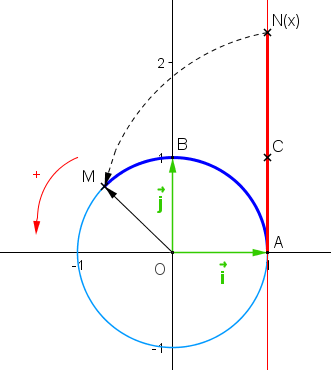
\includegraphics[scale=0.55]{01-02-02.png}
    \end{minipage}
    
    \vspace{-1cm}
    \subsection{Le radian}
    
    La longueur du cercle trigonométrique est égale à $2\pi$.\\
    En effet, son rayon est 1 donc $P = 2\pi R = 2\pi \times 1 = 2\pi$\\
    Ainsi, à un tour complet sur le cercle, on peut faire correspondre le nombre réel $2\pi$.\\
    On définit alors une nouvelle unité d'angle : le radian, tel qu'un tour complet mesure 360\degree ou $2\pi$ radians.

    \begin{bdefi}
        On appelle \grasInDef{radian}, noté rad, la mesure de l'angle au centre qui intercepte un arc de longueur 1 du cercle.
        \begin{center}
        \psset{xunit=0.5cm,yunit=0.5cm,algebraic=true,dimen=middle,dotstyle=o,dotsize=5pt 0,linewidth=2.pt,arrowsize=3pt 2,arrowinset=0.25}
        \begin{pspicture*}(-3.5,-3.5)(3.5,3.5)
        \pscircle[linewidth=0.8pt](0.,0.){1.5}
        \pscustom[linewidth=1.2pt,linecolor=ForestGreen,fillcolor=ForestGreen,fillstyle=solid,opacity=0.1]{
        \parametricplot{0.0}{1.0077885168662493}{0.6*cos(t)+0.|0.6*sin(t)+0.}
        \lineto(0.,0.)\closepath}
        \psline[linewidth=1.2pt,linecolor=red](0.,0.)(3.,0.)
        \parametricplot[linewidth=1.2pt,linecolor=red]{0.0}{1.0077885168662493}{1.*3.*cos(t)+0.*3.*sin(t)+0.|0.*3.*cos(t)+1.*3.*sin(t)+0.}
        \psline[linewidth=1.2pt](0.,0.)(1.6011965208465855,2.5369607213413436)
        \begin{scriptsize}
        \psdots[dotsize=4pt 0,dotstyle=*,linecolor=darkgray](0.,0.)
        \rput[bl](-0.52,-0.42){\darkgray{$O$}}
        \rput[bl](1.48,-0.42){\red{1}}
        \rput[bl](2.74,1.58){\red{1}}
        \rput[bl](0.64,0.2){\textcolor{ForestGreen}{1 rad}}
        \end{scriptsize}
        \end{pspicture*}
        %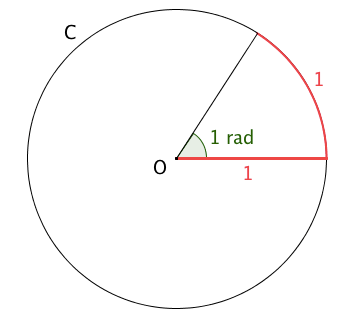
\includegraphics[scale=0.35]{01-02-03.png}
        \end{center}
    \end{bdefi}
    
    \subsection{Correspondance degrés et radians}
    
    Ainsi, à $2\pi$ radians (tour complet), on fait correspondre un angle de $360\degree$.\\
    Par proportionnalité, on obtient les correspondances suivantes :\\
    \ \\
    \begin{tabular}{ | Xc | Xc | Xc | Xc | Xc | Xc | Xc | Xc |}
         \hline			
           \rowcolor{NavyBlue!55!white}Angle en degrée($\degree$)  & 0 & 30 & 45 & 60 & 90 & 180 & 360 \\ \hline
           \rowcolor{NavyBlue!25!white}Angle en radian & $0$ & $\dfrac{\pi}{6}$ & $\dfrac{\pi}{4}$ & $\dfrac{\pi}{3}$ & $\dfrac{\pi}{2}$ & $\pi$ & $2\pi$ \\
         \hline  
    \end{tabular}
    
    \begin{bmethodet}{Passer des degrés aux radians et réciproquement}
        \grasInMet{Enoncé :}
        \begin{enumMet}
            \item Donner la mesure en radians de l'angle $\alpha$ de mesure $33\degree$.
            \item Donner la mesure en degrés de l'angle $\beta$ de mesure $\dfrac{3\pi}{8}$ rad.
        \end{enumMet}
    \end{bmethodet}
    
\section{Mesure d'un angle orienté}

    \subsection{Plusieurs enroulements de la droite}
        \begin{minipage}{0.75\linewidth}
            A plusieurs points de la droite orientée on peut faire correspondre un même point du cercle. La droite orientée peut en effet s'enrouler plusieurs fois autour du cercle dans un sens et dans l'autre.\\
            \begin{bexemples}
            \begin{itemEx}
                \item Ci-contre, les points $N$ et $P$ d'abscisses $\dfrac{3\pi}{4}$ et $-\dfrac{5\pi}{4}$ correspondent tous les deux au point $M$.\\ 
                En effet : $\dfrac{3\pi}{4} -2\pi= -\dfrac{5\pi}{4}$
                \item On pourrait poursuivre le processus dans l'autre sens en effectuant 1, 2, 3, ... tours successifs.\\ 
                % Ainsi, les points d'abscisses $\dfrac{3\pi}{4}$ et $\dfrac{19\pi}{4}$ correspondent au point $M$.\\ 
                % En effet : $\dfrac{3\pi}{4} +4\pi= \dfrac{19\pi}{4}$.
            \end{itemEx}
        \end{bexemples}
        \end{minipage} \hfill
        \begin{minipage}{0.25\linewidth}
            \begin{center}
                \newrgbcolor{qqzzqq}{0. 0.6 0.}
                \newrgbcolor{xfqqff}{0.4980392156862745 0. 1.}
                \psset{xunit=1cm,yunit=1cm,algebraic=true,dimen=middle,dotstyle=o,dotsize=8pt 0,linewidth=0.8pt,arrowsize=3pt 2,arrowinset=0.25}
                \begin{pspicture*}(-2.,-4.5)(2.5,2.3)
                \psaxes[labelFontSize=\scriptstyle,xAxis=true,yAxis=true,labels=none,Dx=1.,Dy=1.,ticksize=-2pt 0,subticks=2]{->}(0,0)(-2.,-4.5)(2.5,2.3)
                \pspolygon[linewidth=1.2pt,fillcolor=black,fillstyle=solid,opacity=1](-0.5066933483806594,0.862126354258351)(-0.42451275812065586,0.9172810429953469)(-0.5054792770152563,0.957764302442647)
                \pspolygon[linewidth=1.2pt,fillcolor=black,fillstyle=solid,opacity=1](-0.5066933483806594,0.862126354258351)(-0.5521299533927227,0.7798135579819784)(-0.6067341821145836,0.8400182204189017)
                \pscircle[linewidth=0.8pt,linecolor=qqzzqq](0.,0.){1.}
                \parametricplot[linewidth=1.2pt,linecolor=red]{2.3320450984702887}{2.872851867759325}{1.*1.2850666792859502*cos(t)+0.*1.2850666792859502*sin(t)+0.|0.*1.2850666792859502*cos(t)+1.*1.2850666792859502*sin(t)+0.}
                \psline[linewidth=1.pt,linecolor=blue]{->}(0.,0.)(1.,0.)
                \psline[linewidth=1.pt,linecolor=blue]{->}(0.,0.)(0.,1.)
                \rput[tl](0.422451499927241,0.1348897567913225){$\blue{\vec{i}}$}
                \rput[tl](-0.18368461700829827,0.7042903514883441){$\blue{\vec{j}}$}
                \psline[linewidth=1.2pt,linecolor=red](-1.238940501289754,0.34120786109776535)(-1.1566043604374026,0.4103524734956868)
                \psline[linewidth=1.2pt,linecolor=red](-1.238940501289754,0.34120786109776535)(-1.264657109699034,0.4373656608110946)
                \rput[tl](-1.1939114785675304,0.9063357238001903){\red{+}}
                \psline[linewidth=0.8pt](1.,-4.5)(1.,2.3)
                \parametricplot[linewidth=1.2pt,linestyle=dashed,dash=2pt 2pt]{1.5413461266504365}{2.7472202756000637}{1.*1.5815250404268189*cos(t)+0.*1.5815250404268189*sin(t)+0.9534305034388083|0.*1.5815250404268189*cos(t)+1.*1.5815250404268189*sin(t)+0.2544588540208172}
                \parametricplot[linewidth=1.2pt,linecolor=red]{0.0}{2.1021413143570626}{1.*1.*cos(t)+0.*1.*sin(t)+0.|0.*1.*cos(t)+1.*1.*sin(t)+0.}
                \psline[linewidth=1.2pt]{->}(0.,0.)(-0.5066933483806594,0.862126354258351)
                \psline[linewidth=1.2pt,linecolor=red](1.,0.)(1.,1.8352981043834493)
                \psline[linewidth=1.2pt,linecolor=xfqqff](1.,0.)(1.,-3.74336104493671)
                \parametricplot[linewidth=1.2pt,linecolor=xfqqff]{-4.181043992822524}{0.0}{1.*1.*cos(t)+0.*1.*sin(t)+0.|0.*1.*cos(t)+1.*1.*sin(t)+0.}
                \parametricplot[linewidth=1.2pt,linestyle=dashed,dash=2pt 2pt]{2.1610272289783277}{4.754511813416839}{1.*2.5167627116062086*cos(t)+0.*2.5167627116062086*sin(t)+0.8940181721833393|0.*2.5167627116062086*cos(t)+1.*2.5167627116062086*sin(t)+-1.2288307908526448}
                \psline[linewidth=1.2pt](-0.5066933483806594,0.862126354258351)(-0.42451275812065586,0.9172810429953469)
                \psline[linewidth=1.2pt](-0.42451275812065586,0.9172810429953469)(-0.5054792770152563,0.957764302442647)
                \psline[linewidth=1.2pt](-0.5054792770152563,0.957764302442647)(-0.5066933483806594,0.862126354258351)
                \psline[linewidth=1.2pt](-0.5066933483806594,0.862126354258351)(-0.5521299533927227,0.7798135579819784)
                \psline[linewidth=1.2pt](-0.5521299533927227,0.7798135579819784)(-0.6067341821145836,0.8400182204189017)
                \psline[linewidth=1.2pt](-0.6067341821145836,0.8400182204189017)(-0.5066933483806594,0.862126354258351)
                \begin{scriptsize}
                %\psdots[dotsize=1pt 0,dotstyle=*,linecolor=darkgray](0.,0.)
                \rput[bl](-0.47756879491643855,-0.37940755454792274){\darkgray{$O$}}
                %\psdots[dotsize=1pt 0,dotstyle=*,linecolor=darkgray](1.,0.)
                \rput[bl](1.0653231391012978,0.15325751791058126){\darkgray{$A$}}
                \psdots[dotstyle=x](-0.5066933483806594,0.862126354258351)
                \rput[bl](-0.7347174505860613,1.071645573873519){$M$}
                \psdots[dotstyle=x](1.,1.8352981043834493)
                \rput[bl](1.17,1.53){$N\left(\dfrac{3\pi}{4}\right)$}
                \psdots[dotstyle=x](1.,-3.74336104493671)
                \rput[bl](1.0653231391012978,-3.557030228179688){$P\left(-\dfrac{5\pi}{4}\right)$}
                \end{scriptsize}
                \end{pspicture*}
                %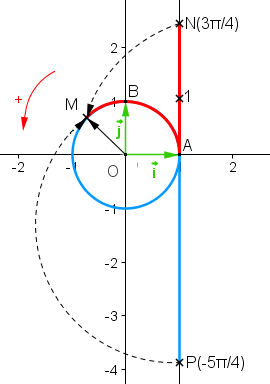
\includegraphics[scale=0.65]{01-02-04.png}
            \end{center}
        \end{minipage}
        
        
        \begin{bmethodet}{Placer un point sur le cercle trigonométrique}
            \grasInMet{Enoncé :}
            \begin{enumMet}
                \item Placer sur le cercle trigonométrique, le point $M$ tel que l'angle $(\vv{i}  ;\vv{OM} )$ mesure $\dfrac{9\pi}{4}$ rad.
                \item Placer sur le cercle trigonométrique, le point $N$ tel que l'angle $(\vv{i}  ;\vv{ON} )$ mesure $\dfrac{8\pi}{3}$ rad.
            \end{enumMet}
        \end{bmethodet}
        
        
        
            
        
    \subsection{Mesure principale d'un angle orienté }
    
        On a vu qu'un angle possède plusieurs mesures.\\
        Si $\theta$ est une mesure de l'angle  $(\vv{i}  ;\vv{OM} )$ alors tout angle de la forme $\theta+k\times2\pi$, avec $k\in \Z$, est une mesure de l'angle $(\vv{i}  ;\vv{OM} )$.\\
        On dit que l'angle $(\vv{i}  ;\vv{OM} )$ est égal à $\theta$ modulo $2\pi$.
        \begin{spacing}{1.7}
        \begin{bdefi}
            \pointille[\textwidth]
            \pointille[\textwidth]
        \end{bdefi}
    	\end{spacing}
        
        \begin{bexemple}
            Une mesure d'un angle orienté est $\dfrac{7\pi}{4}$.\\
            D'autres mesures sont : $\dfrac{7\pi}{4}-2\pi$; $\dfrac{7\pi}{4}-4\pi$; $\dfrac{7\pi}{4}-6\pi$; ... soit : $-\dfrac{\pi}{4}$ ; $-\dfrac{9\pi}{4}$ ; $-\dfrac{17\pi}{4}$ ; ...\\
            $-\dfrac{\pi}{4}$ est la mesure principale de cet angle orienté car c'est la seule comprise entre $-\pi$ exclu et $\pi$.
        \end{bexemple}
        
        \begin{bmethodet}{Donner la mesure principale d'un angle}
            \grasInMet{Enoncé :}\\
            Donner la mesure principale de l'angle $\dfrac{27\pi}{4}$.\\ 
        \end{bmethodet}
\vspace{-1cm}
\section{Cosinus et sinus d'un angle}
    \subsection{Définitions}
    
        \begin{minipage}{0.55\linewidth}
            Dans le plan muni d'un repère orthonormé \Rij et orienté dans le sens direct, on considère un cercle trigonométrique de centre $O$.\\
            Pour tout nombre réel $x$, considérons le point $N$ de la droite orientée d'abscisse $x$.\\ 
            À ce point, on fait correspondre un point $M$ sur le cercle trigonométrique.\\
            On appelle $H$ et $K$ les pieds respectifs des perpendiculaires à l'axe des abscisses et à l'axe des ordonnées passant par $M$.
        \end{minipage} \hfill
        \begin{minipage}{0.45\linewidth}
            \begin{center}
                \newrgbcolor{xfqqff}{0.4980392156862745 0. 1.}
                \newrgbcolor{qqzzqq}{0. 0.6 0.}
                \psset{xunit=2cm,yunit=2cm,algebraic=true,dimen=middle,dotstyle=o,dotsize=8pt 0,linewidth=0.8pt,arrowsize=3pt 2,arrowinset=0.25}
                \begin{pspicture*}(-1.5,-1.2)(1.5,1.2)
                \psaxes[labelFontSize=\scriptstyle,xAxis=true,yAxis=true,labels=none,Dx=1,Dy=1,ticksize=-2pt 0,subticks=1]{->}(0,0)(-1.5,-1.2)(1.5,1.2)
                \pspolygon[linewidth=1.2pt,linecolor=red,fillcolor=red,fillstyle=solid,opacity=1](0.40977974882738943,0.4381983185914975)(0.41741048167754885,0.4184481865087321)(0.4281832809954209,0.43191418565607215)
                \pscircle[linewidth=0.8pt](0.,0.){2}
                \parametricplot[linewidth=1.2pt,linecolor=red]{2.3320450984702887}{2.872851867759325}{1.*1.2850666792859502*cos(t)+0.*1.2850666792859502*sin(t)+0.|0.*1.2850666792859502*cos(t)+1.*1.2850666792859502*sin(t)+0.}
                \psline[linewidth=1.2pt,linecolor=blue]{->}(0.,0.)(1.,0.)
                \psline[linewidth=1.2pt,linecolor=blue]{->}(0.,0.)(0.,1.)
                \rput[tl](0.7,-0.05){\scriptsize $\blue{\vv{i}}$}
                \rput[tl](-0.2,0.88){\scriptsize $\blue{\vv{j}}$}
                \psline[linewidth=1.2pt,linecolor=red](-1.238940501289754,0.34120786109776535)(-1.1566043604374026,0.4103524734956868)
                \psline[linewidth=1.2pt,linecolor=red](-1.238940501289754,0.34120786109776535)(-1.264657109699034,0.4373656608110946)
                \rput[tl](-1.22,0.74){\red{+}}
                \psline[linewidth=0.8pt](1.,-1.2)(1.,1.2)
                \parametricplot[linewidth=0.8pt,linestyle=dashed,dash=1pt 1pt]{1.7070104914828212}{1.989170336710919}{1.*1.1703098632121625*cos(t)+0.*1.1703098632121625*sin(t)+1.1589202721830498|0.*1.1703098632121625*cos(t)+1.*1.1703098632121625*sin(t)+-0.3393763856576485}
                \parametricplot[linewidth=1.2pt,linecolor=red]{0.0}{0.8183148200277329}{1.*1.*cos(t)+0.*1.*sin(t)+0.|0.*1.*cos(t)+1.*1.*sin(t)+0.}
                \psline[linewidth=1.2pt]{->}(0.,0.)(0.6834523503170895,0.7299951265906138)
                \psline[linewidth=1.2pt,linecolor=red](1.,0.)(1.,0.8200931150283057)
                \parametricplot[linewidth=1.2pt,linecolor=red]{0.0}{0.8188989562169464}{1.*0.6*cos(t)+0.*0.6*sin(t)+0.|0.*0.6*cos(t)+1.*0.6*sin(t)+0.}
                \psline[linewidth=1.2pt,linecolor=red](0.40977974882738943,0.4381983185914975)(0.41741048167754885,0.4184481865087321)
                \psline[linewidth=1.2pt,linecolor=red](0.41741048167754885,0.4184481865087321)(0.4281832809954209,0.43191418565607215)
                \psline[linewidth=1.2pt,linecolor=red](0.4281832809954209,0.43191418565607215)(0.40977974882738943,0.4381983185914975)
                \psline[linewidth=0.8pt,linestyle=dashed,dash=1pt 1pt](0.6834523503170895,0.7299951265906138)(0.,0.7283487195713757)
                \psline[linewidth=0.8pt,linestyle=dashed,dash=1pt 1pt](0.6834523503170895,0.7299951265906138)(0.684411097342735,0.)
                \psline[linewidth=1.2pt,linecolor=xfqqff](0.,0.)(0.,0.7283487195713757)
                \psline[linewidth=1.2pt,linecolor=qqzzqq](0.,0.)(0.684411097342735,0.)
                \begin{scriptsize}
                \psdots[dotsize=2pt 0,dotstyle=*,linecolor=darkgray](0.,0.)
                \rput[bl](-0.15,-0.15){\darkgray{$O$}}
                \psdots[dotsize=2pt 0,dotstyle=*,linecolor=darkgray](1.,0.)
                \rput[bl](1.0170341702650048,0.03160536668364699){\darkgray{$A$}}
                \psdots[dotstyle=x](0.6834523503170895,0.7299951265906138)
                \rput[bl](0.6367693438651923,0.7723295597749434){$M$}
                \psdots[dotstyle=x](1.,0.8200931150283057)
                \rput[bl](1.0170341702650048,0.8594735824915666){N(x)}
                \rput[bl](0.573391872798557,0.26530979124186355){\red{x}}
                \psdots[dotsize=2pt 0,dotstyle=*](0.,0.7283487195713757)
                \rput[bl](0.014877909023832495,0.7683684678332788){$K$}
                \psdots[dotsize=2pt 0,dotstyle=*](0.684411097342735,0.)
                \rput[bl](0.7001468149318277,0.03952755056697636){$H$}
                \rput[bl](-0.4,0.35){\xfqqff{sin(x)}}
                \rput[bl](0.24,-0.15){\qqzzqq{cos(x)}}
                \end{scriptsize}
                \end{pspicture*}
                %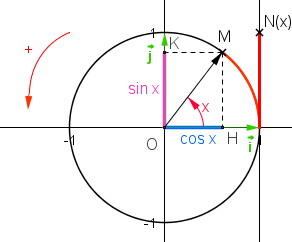
\includegraphics[scale=0.8]{01-02-07.png}
            \end{center}
        \end{minipage}
        
        \begin{spacing}{1.7}
        \begin{bdefis}
            \begin{itemDef}
                \item \pointille[15cm]
                \item \pointille[15cm]
            \end{itemDef}
        \end{bdefis}
    	\end{spacing}
        
    \subsection{Propriétés}
    	\begin{spacing}{1.7}
        \begin{bprops}
            \begin{itemProp}
                \item \pointille[15cm]
                \item \pointille[15cm]
                \item \pointille[15cm]
                \item \pointille[15cm]
                \item \pointille[15cm]
            \end{itemProp}
        \end{bprops}
    	\end{spacing}
        
        \begin{brmq}
            $(\sin x)^2$, par exemple, se note $\sin^2 x$
        \end{brmq}
        
    \subsection{Valeurs remarquables des fonctions sinus et cosinus}
    
        \begin{center}
            \begin{tabular}{ | Xc | Xc | Xc | Xc | Xc | Xc | Xc |}
                 \hline			
                   \rowcolor{NavyBlue!55!white}$x$  & $0$ & $\dfrac{\pi}{6}$ & $\dfrac{\pi}{4}$ & $\dfrac{\pi}{3}$ & $\dfrac{\pi}{2}$ & $\pi$ \\ \hline
                   \rowcolor{NavyBlue!25!white}$\cos x$ & $1$ & $\dfrac{\sqrt 3}{2}$ & $\dfrac{\sqrt 2}{2}$ & $\dfrac{1}{2}$ & $0$ & $-1$ \\ \hline
                   \rowcolor{NavyBlue!25!white}$\sin x$ & $0$ & $\dfrac{1}{2}$ & $\dfrac{\sqrt 2}{2}$ & $\dfrac{\sqrt 3}{2}$ & $1$ & $0$ \\
                 \hline  
            \end{tabular}
        \end{center}
    
    \subsection{Cosinus et sinus d'angles associés}
    
        \begin{spacing}{1.7}
        	\begin{bprops}
            Pour tout nombre réel $x$, on a :
            \begin{enumProp}
                \item \pointille[15cm]
                \item \pointille[15cm]
                \item \pointille[15cm]
                \item \pointille[15cm]
            \end{enumProp}
        \end{bprops}
    \end{spacing}
        
        \begin{bdemo}
                On démontre les résultats par des symétries:
        \end{bdemo}
        
